\chapter{深層学習による病理画像の診断支援}
\label{chap_review}
病理画像をデジタルで保存することが始まったのは数十年前になる.これによって遠隔地でも診断することができるようになったり,情報を共有することができるようになり,複数の医師で診断しミスを防止するsecond opinionが容易になった.計算機科学の分野の側面ではデータを収集することができるようになり,研究が盛んに行われることになった.その後は,様々な病理データでより改良されたアルゴリズムの提案が行われている.

細胞組織の形態を観察するための病理染色ではヘマトキシリン・エオジン染色(HE染色)が一般的に用いられる.細胞核を青紫色に染色し,細胞質をピンク色に染色する.正常から異常に変化していくと,細胞核が過度に増殖したり,細胞質の形が崩れたりすることで,その特徴を機械学習によって精度よく検出するための研究が行われている.

これまでは,核の形やテキスチャーからパターンマッチングなどの画像処理によって腫瘍を検出する研究されてきたが,近年になって画像処理に大きなブレークスルーが起きたことをきっかけに,新しい手法で解析するようになってきた.そのブレークスルーがディープラーニングである.

\section{ニューラルネットワーク}
人間の脳にはニューロンと呼ばれる神経細胞が1000億個以上あり,それぞれが複数のニューロンと電気信号で情報を伝達している.また脳には電気信号を受け渡すシナプスという場所がある.ニューロンとシナプスで行われる演算を模倣したアルゴリズムを作ることができれば人間のような思考や認識をコンピュータを使って再現できると考えた.そのアルゴリズムがニューラルネットワークである.

\subsection*{多層パーセプトロン}
ニューラルネットワークは入力層,出力層,隠れ層から構成され,層と層の間にはニューロン同士のつながりの強さを示す重みがある.非線形問題を扱うために 1986 年 Rumelhart によって考案されたのが,パーセプトロンを複数つなぎ合わせ入力と出力以外に隠れた層を持つ多層パーセプトロン (Multi-layerperceptron: MLP) である.

ニューラルネットワークで多層パーセプトロンの層を全結合(fully connected: FC) 層とも呼ぶ.Figure 3.1 における丸や矢印はそれぞれノード (またはニューロン) と重み (または結合) と呼び,ともに数値である.例えば画像を分類しようと思えば,各ピクセルの画素数を各ノードに入力する (28×28pix のグレースケール画像であれば 784 個のノードが必要).データが入力層に入ってくると,その値に重みをかけ,活性化関数と呼ばれる関数を通し結果を出力する.これを繰り返し出力層に書き出す.各層の重みの値によって出力結果は異なってくる.出力層のノードは区別したいクラス数分用意し,各ノードの出力値が各クラスに属している確率を表す.学習については誤差逆伝播法を利用する.ニューラルネットワークの出力値と正解データとの比較をした時に,どれだけ正解から離れているかを評価する損失関数 (Loss) を使って,損失関数が小さくなるようにノード間の重みを勾配降下法によって更新する.

\subsection*{畳み込みニューラルネットワーク}
畳み込みニューラルネットワーク (ConvolutionalNeural Network: CNN) は,1998 年には既に LeNetと呼ばれるネットワークで実装されていた [3].従来の画像認識では,画像から特徴を抽出し,それをニューラルネットワークにかけるいわゆる特徴量設計が必要で,ここをいかにうまく設計するかがポイントであったが,CNN は特徴量設計から識別までを end-to-end で行うことがきることが最大の強みである.人間が物体を認識することをコンピュータにも計算させるには,画像の特徴的な部分を切り分けて数値化させる必要がある.例えば,カラー画像の場合,RGB の 3 色 (3 チャンネル)を組み合わせた画像で認識をしている.このようなフィルターの畳み込み計算を行うと,フィルターごとに異なった画像の特徴を抽出して数値化する.これが畳み込み (convolution) である.その後,画像のサイズを小さくしてコンピュータが計算コストを減らし,微小な変化に対してロバストになる仕組みしてプーリングという方法を用いる.学習には MLPと同様に誤差逆伝播法を用いる.

\section{画像認識におけるディープラーニング}
ディープラーニングが注目を受けることになったのは、2012の画像認識コンペティションであるILSVCでHintonがAlexNetというDeepLearningの手法で他のチームを圧倒する精度を出したことが始まりである.

ディープラーニングは、その名の通り、今までのニューラルネットワークよりも層が深くなっている。この層の深さが、より複雑な特徴を抽出することができる。層の深さはモデル設計でチューニングしていく必要があり、上述のAlexNetは8層のネットワークであった。しかし、ネットワークの層は深くなっていき、現在では152層のResNetというものがILSVC2015でもっとも精度が良く、人間の認識精度を超えている。ディープラーニングによる学習方法について、畳み込みニューラルネットワーク(Convolutional Neural Network : CNN)を利用する。入力する画像に対して小さなサイズ(3×3など)のフィルターを畳み込み計算をする。このフィルターの値を学習することがディープラーニングの学習である。フィルターの数も設計する必要がある。学習については、誤差逆伝播法を利用する。ディープラーニングの出力結果と正解との比較をした時に、どれだけ正解から離れているかを評価する誤差関数を使って、その誤差関数が小さくなるように、フィルターの重みを変更する時に勾配降下法を使う。

Deep Learning とは Deep Neural Network(DNN)を指すことが多い.この"Deep"とは,ニューラルネットワークの層が深いことに由来している.
Figure 3.3 に画像認識タスクの精度の近年の推移を示す.これは ImageNet Large Scale Visual RecognitionChallenge (ILSVRC) と呼ばれる世界的な画像認識のコンペティションである (2010 年から始まった).カテゴリ数は 1000 クラスで,画像枚数は120 万枚の訓練データと 15 万枚のテストデータが用意されている.2011 年と 2012 年は約 10\%もの大差で AlexNet[4] が優勝している.これがディープラーニングの始まりである.AlexNet は 5 つの畳み込み層と 3 つの全結合層を持っている.2014 年には VGGNet[5] や GoogLeNet[6] が 9 割の精度を超えた.VGGNet は AlexNet(8 層) よりさらに深い構造(19 層) であり,GoogLeNet は 22 層もある.そして2015 年には ResNet[7] が人間の精度をも超える認識精度を達成した.ResNet は GoogLeNet よりもさらに深く 152 層もある.一般に,層を深くすることは簡単ではなく,勾配消失や過学習といった問題が起こる.それの対策として様々な手法が用いられている.

画像処理におけるディープラーニングができることは、画像から(1)カテゴリ分けをすること、(2)物体を検出すること、(3)物体のセグメンテーションをすることである.

CNNを複数回かけて検出を行う場合、CNNの浅い側では空間分解能はあるが抽象的な情報が少ない。深い側では意味論的な情報は取得できる(ポーズ、変形など) が空間分解能が小さいため幾何学的な情報が失われる。

位置情報を含むデータセットで事前学習することで精度が上がることが示されている。当然ながらこの場合事前学習のデータセットと適用データとの間に類似性があると良い。

アーキテクチャの進化の方向は①層が深くなること ②FC層の使用を避けること又はInceptionモジュールの使用によってパラメータ数を削減すること ③ ResNetなどのショートカット接続によって学習効率をあげること

\subsection*{事前学習 / 転移学習}

\subsection*{物体検出}
物体検出とはBounding Boxで物体の位置とその物体の種類を特定する方法である.歴史的には幾何的情報,手動特徴量,そしてそのカスケードを利用していた.その後,HOGやSIFTなど局所特徴量を抽出する方法を設計するようになったが、これは深い専門知識を必要とした.また広い範囲でオブジェクトを正確に検出する方法は、メモリ容量と処理時間に課題がある.現在はDeep Neural Networkになりデータのみから抽象的な特徴量を複数得ることができる。一般物体認識の場合は数千のカテゴリを学習してTop Error Rateが2\%以下と人間よりも認識精度が高いが,物体検出においては,今はカテゴリがせいぜい数百程度くらいまででも認識精度が人間よりも低くなってしまう.また物体検出は精度を上げるために処理に時間がかかるアルゴリズムであることが多いため,リアルタイムに物体検出を行う時は,速度と精度でトレードオフが生じてしまう.

\begin{figure}[h]
\centering
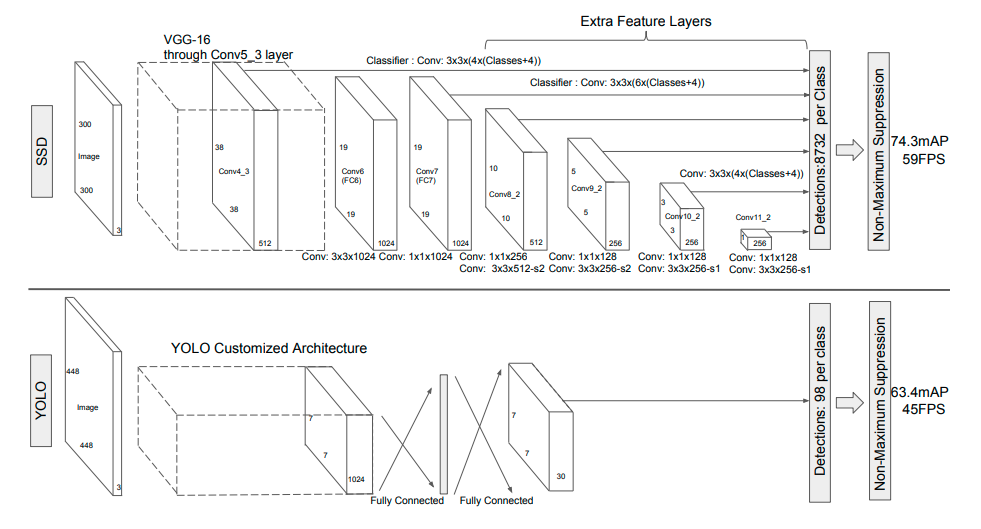
\includegraphics[width=0.7\linewidth]{fig/yolo_ssd.png}
\end{figure}

\subsection*{セマンティックセグメンテーション}
セマンティックセグメンテーションとは,画像を画素レベルで認識することである.画像内の各画素をオブジェクトクラスに割り当てる手法である.セマンティックセグメンテーションの手法についてディープラーニング以前では,Texton Forestsや,Random Forestsに基づいた分類を行っていたけれど物体検出と同様にCNNが登場してからは,高精度なセグメンテーションが実現するようになった.CNNを使ったセグメンテーションの手法で一般的に使われるようになったものがUnetである.このUnetは文字通りUの形をしたネットワークであることが特徴で,2つのアーキテクチャーからできている.一つ目がエンコーダーのアーキテクチャーでCNNとプーリングで特徴を抽出しながら次元を削減していき,2つ目のデコーダーのアーキテクチャーで画像をセグメンテーションの結果になるように復元する.ここで問題になることが,プーリングをすることで位置情報を消してしまっているので,この位置情報を利用して画像を復元するためには,エンコーダーとデコーダーで画像サイズが同じところ同士をショートカットで接続することがUnet構造の優れている点である.

\begin{figure}[h]
\centering
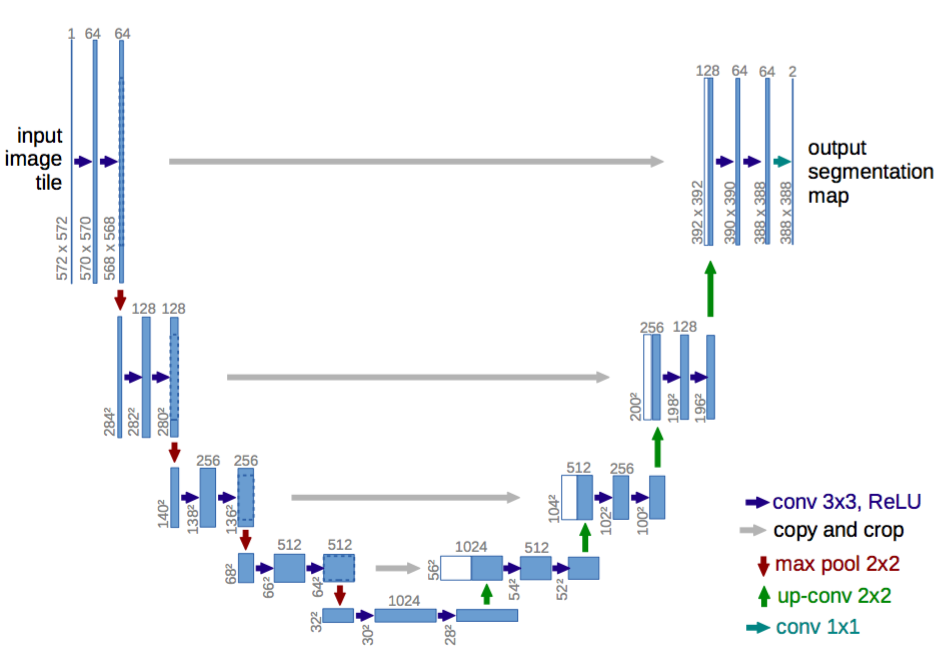
\includegraphics[width=0.7\linewidth]{fig/unet.png}
\end{figure}

\subsection*{深層学習による3次元画像解析}

\section{教師なし学習}

\section{半教師あり学習}

\section{ディープラーニングを用いた病理画像診断}
学習した結果を評価するときに医療画像の場合は、PrecisionとRecallを識別性能の評価指数として使う。

\begin{align}
  \mathrm{Precision} & = \dfrac{TP}{TP+FP}\\
  \mathrm{Recall} & = \dfrac{TP}{TP+FN}
\end{align}

ここで使ったTP(True Positive)は真の結果が正である時に予測も正であるという意味であるTN(True Negative)は真の結果が正で予測が負である場合である。同様にFP(False Positive)真の結果が負で予測も負、FN(False Negative)真の結果が負で予測は正である.

2016年に行われたCAMELYON16という乳がんの転移を調べるシステムのコンペティションでは、7人の医師の成績を上回っていることが報告されてている。

また皮膚癌の種類が757種類を細かい違いまで識別するように学習する。学習方法はInception v3というネットワークを利用している。これは22層の畳み込みニューラルネットワークである。またこのネットワークは皮膚癌の識別タスクを学習する前に、IMageNetというILSVCでも使っている一般物体画像を使って事前にネットワークの重みの初期値を決めることによって、精度が向上させる。これを転移学習(Transfer Learning)と呼ばれている。
